\documentclass[11pt,a4paper]{article}
\setlength{\headheight}{34pt}
\usepackage[export]{adjustbox}
\renewcommand{\baselinestretch}{1.3}\normalsize
\usepackage[margin=1.2in]{geometry}
\usepackage[T1]{fontenc}
\usepackage[utf8]{inputenc}
\usepackage[german]{babel}
\usepackage[printonlyused]{acronym}
\usepackage[
	colorlinks=false,
	urlcolor=blue,
	linkcolor= gray
]{hyperref}
\usepackage{lmodern,textcomp}
\usepackage{graphicx}
\usepackage{appendix}
\usepackage{pdfpages}
\usepackage{listings}
\graphicspath{ {images/} }
\usepackage{amsmath}
\usepackage{svg}
\usepackage{amsfonts}
\usepackage{amssymb}
\usepackage{fancyhdr}
\pagestyle{fancy}
\usepackage{lscape}
\fancyhf{}
\rhead{
\includegraphics[scale=0.05]{logo_zmb}}
\lhead{\textbf{Agentur Website}\\Ein Full Stack Webdevelopement Projekt}
\rfoot{Seite \thepage}
\author{Jeremy Seipelt}
\title{IHK Abschluss-Projekt 2017}
\begin{document}
\clearpage\maketitle
\thispagestyle{empty}
	\begin{center}
		\begin{Large}


			Für den Beruf des Fachinformatiker der Anwendungsentwicklung\\

		\end{Large}
	\end{center}

 	\begin{center}
		\begin{LARGE}
			 \textbf{Agentur Website}\\
		 Ein Full-Stack Web-Developer Projekt
		\end{LARGE}
	\end{center}

	\begin{center}
	Auszubbildner: \\
 	Jeremy Seipelt\\
 	Pichelsdorferstr. 72\\
	 13595 Berlin\\
	\end{center}

	\begin{center}
		
\includegraphics[scale=0.05]{logo_zmb}\\
 		Ausbildungsbetrieb:\\
 		zmb GmbH\\
 		Scharnhorstr. 112\\
 		11234 Berlin \\
 	\end{center}
\newpage
\tableofcontents
\newpage
\begin{acronym}[Full Stack]
 \acro{SSR}{Server Sided Rendering}
 \acro{SPA}{Single Page Application}
 \acro{DOM}{Document Object Model}
 \acro{CMS}{Content Management System}
 \acro{AOT}{Ahead of time}
 \acro{REST}{Representational State Transfer}
 \acro{SASS}{Super Awsome Style Sheets}
 \acro{API}{Application Programming Interface}
 \acro{JSON}{Javascript Object Notation}
 \acro{UI}{User Interface}



\end{acronym}
\begin{acronym}[Allgemein]
 \acro{B2B}{Business to Business}
 \acro{KMU}{Kleines Mittelständisches Unternehmen}
\end{acronym}
\newpage
\pagenumbering{arabic}
\setcounter{page}{1}
\section{Vorwort}
Diese Projektdokumentation ist für die Abschlussprüfung der IHK für den Beruf des Fachinformatikers der Anwendungsentwicklung entstanden und beschreibt Vorgehensweisen des Verfassers.\\
Ausbildungsbetrieb ist die zmb GmbH, ein \acs{KMU} mit Standort in Berlin Mitte.
Die zmb vertreibt, supportet, und entwickelt ihre eigene E-Commerce Plattform, genannt CORE, und geht Projektarbeiten im \acs{B2B} Bereich für alle gängigen Shopsysteme nach.
Dabei legt die zmb Wert darauf alle Wünsche des Kunden, von der Bereitstellung eigener API über Onboarding bis hin zu Zahlungsweisen, zu erfüllen. Dem Kunden werden auch individuelle Lösungen angeboten.
\subsection{Beschreibung des Projektes}
Für die Agenturarbeiten der zmb, soll eine neue Internet-Präsenz aufgebaut werden.\\\\\\
Die neue Seite wird eine \acs{SPA} um die Seite für den Kunden modern und schnell zu machen.
Der Server muss dafür die \acs{SPA} bereits kompiliert versenden, da Suchmaschinen sich nur die gesendete HTML Datei ansehen. wird ein \acs{SSR}-Setup auf dem Server benötigt.
Im Verlaufe des Projekts wird ein Server gemietet, aufgesetzt und eine Website erstellt auf der potentielle Kunden mit der zmb in Kontakt treten können.
\subsection{Ziel des Projektes}
Am Ende des Projekts soll eine \acs{SPA} entstehen die mithilfe von \acs{SSR} auch ein hohes SEO Ranking erreicht wird. Dabei sollen namenhafte Geschwindigkeitsindexe die Seite mit maximalen Punkten bewerten.
Die Inhalte der \acs{SPA} werden über ein selbst auf dem Server installiertes CMS-System eingetragen.
Am Ende entsteht eine Website die auch ohne Hilfe von HTML sowie JS und CSS gepflegt werden kann.
\subsection{Umfeld des Projektes}
Das Projekt wurde vom COO Simeon Gerodetti beantragt.\\
Herr Simeon Gerodetti ist in der zmb für das operative Geschäft, für das Marketing und den Online-Auftritt der zmb zuständig.
Des weiteren kümmert er sich um die Partner im \acs{B2B} Bereich, sorgt für Kundenaufträge des Unternehmens.\\\\
Jovan Gerodetti ist der Softwareentwickler für Frontend, sowie der Spezialist in Angular. Er baut neue UIs, Schnittstellen für CORE und stellt eine Beratende Funktion für das Projekt dar.\\\\
Für das Projekt sind die Zuständigkeiten wie folgt:\\
- Simeon Gerodetti für Design\\
- Jovan Gerodett für Implementierung\\\\
- die Abnahme des Projektes wird von Simeon Gerodetti vollzogen.
\subsection{Projektentscheidung}
Das Hauptgeschäft besteht aus dem Verkauf und der Entwicklung der Inhouse E-Commerce Lösung 'CORE', welche von 3 Personen gewartet wird. 'Core' wird bisher nur als SaaS Lösung eingesetzt und deshalb liegt der administrative Aufwand bei der zmb.\\\\
Den weiteren Schritt in die Richtung der Agenturarbeit geht die zmb mit der zmb.agency Website, dessen Unterbau durch dieses Projekt entsteht.
\subsection{Beschränkungen des Projektes}
Das Projekt beschränkt sich auf das Aufsetzen, sowie das Implementieren einer kleineren Version der Agentur Website, die schon alle technischen Voraussetzungen und ein Bruchteil des Inhaltes enthält. Deswegen wird der Großteil der Layout und CSS Arbeiten, die im größeren Umfang ein Teil sind, das Anlegen von Inhalten für die Seite nicht in die Projektzeit eingerechnet.
\section{Projekt-Planung}
Das Projekt wurde auf 70h für die Anforderungen der IHK angesetzt.
\subsection{Projektverlauf}
Ein Übersicht der Hauptphasen sind der Tabelle 1 zu entnehmen. Eine detaillierte Ansicht der Zeitplanung ist in der \ref{sec:teilaufg} auf Seite \pageref{sec:teilaufg} hinterlegt.\\
\begin{table}[!ht]
  \centering
     \begin{tabular}{l|r}
       \textbf{Phase}  & \textbf{Dauer in Stunden} \\
       \hline
      Analyse       & 8                     \\
      Entwurf       & 7             	    \\
      Implementierung       & 23	\\
      Testen       & 13			         \\
       Dokumentation      &  8        \\
       \\
       \hline
       \hline
       Gesammt        & 64               \\
     \end{tabular}
     \caption{Übersicht der Zeitplanung}
\label{tbl:Übersicht der Zeitplanung}
\end{table}
\subsection{Ressourcenplanung}
Bei der Auswahl der Ressourcen wurde Wert auf Open Source Lösungen gelegt, um Projektkosten möglichst gering zu halten. Die Liste der benutzten Software ist aufSeite \pageref{sec:progs}
zu finden.
\subsection{Entwicklungsprozess}
Die Entwicklung der Website wird per Wasserfall-Modell abgewickelt. Dabei werden die einzelnen Phasen des Projektverlaufs nacheinander durchlaufen. Nach jeder Phase wird mit Simeon Gerodetti Rücksprache über den Stand der Dinge gehalten, Jovan Gerodetti übernimmt dessen Rolle in der Implementierung.\\
Das Wasserfall-Modell bietet sich für kleine Software-Projekte an, die einen klaren Endzustand haben. Da die Anforderungen schon niedergeschrieben sind, können diese in der Entwurfsphase mit einbezogen werden. \\\\
Eine Agile Entwicklung ist somit nicht Sinnvoll, und würde nur den Aufwand erhöhen.
\section{Analysephase}
\subsection{Ist-Analyse}
Die zmb ist nur als Firma für den Vertrieb und Wartung von Shop Systemen bekannt, allen voran ihr eigenes 'CORE'. Die Seite informiert nicht über die Agenturarbeit, die die zmb anbietet.
Zu Beginn des Projektes steht nur ein gemieteter AWS Server zur Verfügung, der eine minimale Version der Linux Distribution Ubuntu als Betriebssystem nutzt.
\subsection{Wirtschaftlichkeit}
Aufgrund des Umstieges auf Agenturarbeit, muss auch eben diese im Internet beworben werden. Momentan kommen Aufträge nur aus dem Partnernetzwerk und nicht auf dem direkten Weg zur zmb, deswegen ist die neue Internetpräsenz zwangsweise erforderlich.
\subsubsection{Kosten}
Die Ressourcenplanung besteht aus Personal und Sachkosten.\\\\
Für das Projekt werden 3h für Beratung durch einen Senior Developer eingerechnet.\\\\
Für die Entwicklung wird auf Open Source Lösungen gesetzt. Eine genau Liste der Verwendeten Software auf dem Server wird in Tabelle \pageref{sec:progs} aufgelistet
\begin{table}[!ht]
  \centering
     \begin{tabular}{l|r||l|r}
       \textbf{Personalkosten}  & &\textbf{Sachkosten}& \\
       \hline
       Entwickler      &    70*10€ = 700€    &  AWS Lightsail Server      &     5€/mtl\\
       COO    &  2*30€ = 60€               	    &  Domain & 20€/Jahr\\
       Beratung durch Seniorentwickler    &  3*30€ = 90€ & Software Lizenzen & 0€	\\
       \hline
       \hline
       Gesammt Fix& 850€ & Gesammt Monatlich & \textasciitilde 7€  \\
     \end{tabular}
\caption{Kostenplanung}
\label{tbl:Kostenplanung}
\end{table}
\subsubsection{Amortisation}
Die Seite amortisiert sich durch die Anzahl an Stunden Agenturarbeit die durch sie vergeben wurde.
Zur Berechnung der Stunden werden die Kosten aus der Ressourcenplanung genommen. Für Agenturarbeit wird eine  Pauschale von 100 €/h genommen.\\
\begin{equation*}
x = 850 / 100 = 8.5
\end{equation*}
Somit Rechnet sich die Seite bereits nach 9h Agenturarbeit. Das entspricht 9 Kunden im Worst-Case-Szenario die durch die Seite Agenturarbeit buchen.
\subsection{Anforderungen}
Angefordert wurde eine neue Website.\\\\
Diese Websie muss höchste Punktzahl in verschiedenen Tempo Benchmarks bringen, um den Besucher zu zeigen das die zmb modernste Technologien beherrscht.\\\\
Dabei soll eine \acs{SPA} entstehen, damit der Benutzer wenn er auf der Seite navigiert nicht den \acs{DOM} bei jedem Request neu berechnen muss.
Zur Erstellung der SPA soll Angular verwendet werden, da es sich hierbei um eine bereits im Unternehmen etabliertes Framework handelt.\\\\
Damit Crawler etc unsere Seite/SPA indexieren können muss die Seite bereits auf dem Server vorgerechnet werden um einen fertigen \acs{DOM} an den Crawler zu senden.
Der Prototyp soll dem Mockup von Simeon Gerodetti ähneln.\\ Das Mockup ist auf Seite \pageref{sec:mock} einzusehen.\\Für den Anfang wird nur das Hero Image, sowie das Kontaktformular auf der Landingpage benötigt.
\subsubsection{SSR PoC}
Zur Analyse gehörte auch der Beweis das der SSR Prozess funktioniert. Die von Angular bereitgestellte Projekt Repo\footnote{https://github.com/angular/universal-starter} konnte den Vorgang des serverseitigen Renderns, zur Zufriedenstellung Jovan Gerodettis, vorzeigen.
\section{Entwurfsphase}
Die Anforderungen verlangen eine Website, dadurch ist die Wahl der Zielplattform der Webbrowser\footnote{Alle Webbrowser ab IE9}. Dabei verwenden wir soviel es geht TypeScript\footnote{https://www.typescriptlang.org/}, da es sich hierbei um eine in der Firma etablierte Sprache handelt. TypeScript wird deswegen sowohl auf Client als auch Server Ebene verwendet und vorher zu JavaScript kompiliert.
\subsection{Server}
Der Server ist ein von Amazon gebuchter Lightsail\footnote{https://amazonlightsail.com/} Server, der über ein Linux OS mit Ubuntu als Distribution verfügt. Die auf Seite \pageref{sec:progs} für den Server markierten Programme sollen auf dem Server installiert werden.
\subsubsection{CMS}
Geplant ist ein CMS System auf dem Server (Drupal) mit Datenbank(MYSQL).\\ Dabei soll für jede Komponente der Website, die auf Seite \pageref{sec:epage}
referenziert wird, ein Inhaltstyp erstellt werden.\\
Die Inhalte sollen über ein REST-Modul in Drupal dann, per REST \acs{API}, für die SPA erreichbar sein.
Diese Inhalte werden in dem JSON\footnote{https://www.json.org/} Format versendet.
Geplant sind vorerst folgende REST Schnittstellen:
\begin{table}[!ht]
  \centering
     \begin{tabular}{l|c}
       \textbf{Schnittstelle}  & \textbf{Endpunkt} \\
       \hline
       Inhalte einer bestimmten Seite & \textbf{export/pages/SEITENNAME} \\
       Inhalte aller Seiten & \textbf{export/pages/all} \\
       Inhalte einer bestimmten Sektion & \textbf{/export/paragraphs/ID} \\
       Inhalte aller Sektionen & \textbf{export/paragraphs/all}\\
       Inhalte der Kopfzeile & \textbf{export/headbar}\\
     \end{tabular}
\caption{REST-API}
\end{table}
\subsubsection{HTTP/HTTPS}
Der Server soll über HTTP/HTTPS erreichbar sein. Der Server muss unterscheiden, ob der Benutzer die Agentur SPA anfragt, oder das CMS System. In Anbetracht der weiteren Entwicklung wurde eine zweite Instanz der Webseite erstellt, um Produktions Website von der Entwicklung Website zu trennen. Deswegen werden auf dem Server folgende Routen eingestellt:
\begin{table}[!ht]
  \centering
     \begin{tabular}{l|c}
       \textbf{Anwendung}  & \textbf{Route} \\
       \hline
       Drupal & \textbf{/drupal}\\
       SPA/Agentur Website & \textbf{/}\\
       SPA/Entwicklung & \textbf{/dev}\\
     \end{tabular}
\caption{Routen}
\end{table}
\subsubsection{Node}
Um Javascript auf einem Server ausführen zu können, muss ein Node Server vorhanden sein.
Der Node Server muss jede auf ihm zeigende Route abfangen und die zugehörige Route der SPA bereitstellen. Hier findet der eigentliche SSR Prozess statt. Dem Node Server wird ganze SPA bereitgestellt. Dafür wird das Express Framework verwendet welches HTTP Anfragen an den Node Server verarbeitet. Damit Node mit der SPA funktioniert muss ein \acs{AOT} Compiler die Anwendung für den Server kompilieren.
\subsection{Single Page Application}
Das Framework welches für die SPA verwendet wird ist Angular\footnote{https://angular.io}, welches die zmb seit Jahren produktiv einsetzt. Bei Angular wird der Fokus auf wiederverwendbare Komponenten gesetzt die, wie native DOM-Element, in das HTML eingebunden werden.\\\\
Dafür wurde der generelle Seiten-Aufbau in der Grafik auf Seite \pageref{sec:epage}
festgelegt. Deswegen werden Komponenten entworfen, die für einzelne Passagen der Website stehen.
Um die Rest-API vom CMS konsumieren zu können, benötigen wir noch ein Service\footnote{https://angular.io/guide/dependency-injection}.
Der Entwurfsplan der SPA ist auf der Seite \pageref{sec:espa} hinterlegt.
\section{Implementierungsphase}
\subsection{Server}
\subsubsection{Aufsetzen des Servers}
Der gebuchte Lightsail Server wird nur mit einer minimalen Installation ausgeliefert. Als erstes werden die benötigten Programme installiert. Dabei werden die unter Server auf Seite \pageref{sec:progs} aufgeführten Programme über den Ubuntu Package Manager apt\footnote{https://wiki.ubuntuusers.de/APT/} installiert. Für die einfache Arbeit mit dem Server wurden symbolische Links auf wichtige Serverressourcen in das Home Verzeichnis des Users angelegt, wie auf dem Sreenshot auf Seite \pageref{sec:ordner} .
\subsubsection{NGINX}
Der HTTPS Teil des Servers wird von NGINX gesteuert. Nach der Installation des NGINX, muss der NGINX Service gestartet werden. Sobald der NGINX läuft kann der Server konfiguriert werden. Da Drupal und Node auf dem selben Server liegen, müssen für beide unterschiedliche Routen in der Konfiguration angelegt werden wie auf Seite \pageref{sec:nginx}. Die komplette NGINX Konfiguration ist im Extra Source Code Anhang vorzufinden.
\subsubsection{CMS}
Nach dem Download von Drupal und der einrichtung von MySQL, wird Drupal über einen Aufruf im Webbrowser installiert. Die benötigten Module wurden eingespielt und die Inhaltstypen angelegt.
Die Inhaltstypen mit ihren Feldern sind auf Seite \pageref{sec:content} ff. zu sehen.\\
Die REST Schnittstelle ist über das REST \acs{UI} Modul von Drupal erstellt worden, ein Screenshot der erstellten Schnittstellen ist auf Seite \pageref{sec:rest} zu sehen.
\subsubsection{Node}
Neben Node wurde noch PM2\footnote{http://pm2.keymetrics.io/} installiert um den Node Prozess bei Abstürzen automatisch neu zu starten. Die Installation von Pm2 sowie aller von der SPA benötigten Pakete erfolgt über den Node Package Manager. Dieser installiert automatisch alle Pakete die als Abhängigkeit  in der \textit{package.json} angegeben wurden.\\ Der Inhalt der package.json ist dem Source Code zu entnehmen.
\subsection{SPA}
Für die SPA wurde zuerst ein Grundgerüst bestehend aus einem Root Modul erstellt.\\
Die Seitenkomponenten werden im Drupal Modul deklariert. Dieses Modul besteht aus mehreren Komponenten und einem Drupal Service.\\\\Die Komponenten der Sektionen bekommen ihre Informationen über die Page Komponente. Über das Angular Data Binding\footnote{https://angular.io/guide/template-syntax\#binding-syntax-an-overview} kann das Template mit den erwarteten Daten im Dekorierer der Komponente eingepflegt werden.\\\\
Jede Komponente bekommt eine eigene \textit{.css} Datei, damit die CSS Regeln nur auf diese greifen. Das Aussehen der Seite wurde in SASS implementiert, welches CSS um Konzepte aus der Programmierung, wie Variablen, erweitert.
Mithilfe der Developer Tools von Google Chrome konnte CSS für die Website erstellt werden, ohne die SPA neu zu kompilieren.\\\\
Die SPA wird für den Client als eine \textit{bundle.js} Datei ausgeliefert mithilfe von Webpack\footnote{https://github.com/webpack/webpack}.
Am Ende wurde noch der Taskrunner Gulp hinzugefügt, damit die benötigten Kommandos zum Bauen der SPA auf ein minimum reduziert werden.\\
Die Einstellungen Gulps sind im Source Code hinterlegt.
\section{Abschlussphase}
In folgenden werden die abschließenden Arbeiten beschrieben die den pagespeed und die responsiveness der SPA behandeln.
\subsection{Pagespeed}
Um den maximalen Pagespeed zu erreichen, musste auf dem Server der Cache und gzip aktiviert werden, die gesendeten Dateien wurden vorher nicht komprimiert oder gecacht.\\ Die Performanz des Audits konnte aufgrund der Limitierungen der benutzen Pakete/Libraries/Frameworks nur auf 69/100(zufriedenstellend) erhöht werden.
\subsection{Responsiveness}
Die Responsiveness der Website sollte durch die Verwendung von relativen Größen sichergestellt werden. Diese Annahme erwies sich jedoch als falsch, denn was auf einem großem Bildschirm groß ist, ist dann auf einem kleinen Bildschirm klein. Deswegen wurde um die Werte adjustieren zu können dem \acs{SASS} feste Breiten, für verschiedene Endgeräte, als Variablen angelegt.\\Die einzelnen Komponenten wurden dann auf Handy/Laptop/Computergröße fein justiert.
\section{Dokumentation}
Die Dokumentation besteht aus zwei Teilen einer Projektdokumentation und einer Entwicklerdokumentation.
\subsection{Projektdokumentation}
Die Projektdokumentation besteht aus einer genauen Beschreibung der für die Ausführung des Projektes benötigten Phasen, sowie Information zur in der Phase benutzten Technologie.
Die Dokumentation wird mit \LaTeX geschrieben um ein einheitliches Layout zu gewähren.
\subsection{Entwickerdokumentation}
Die Entwicklerdokumentation besteht aus einer automatisch generierten Doku unter Verwendung von Compodoc\footnote{https://compodoc.github.io/compodoc/}, welcher alle Informationen aus dem Sourcecode bezieht und diese für Entwickler aufbereitet. Diese Dokumentation ist aus dem Sourcecode für alle Entwickler kompilierbar. Screenshot im Anhang \ref{sec:doku} auf Seite \pageref{sec:doku}.
\section{Endstand}
Das Projekt wurde mit einer funktionstüchtigen Website abgeschlossen. Die Maximale Anzahl an Stunden wurde nicht überschritten und der gesammte Planungs Puffer wurde aufgebraucht. Eine genaue Übersicht der Benötigten Zeit ist auf Seite \pageref{sec:time} zu finden.
\subsection{Ist/Soll-Zustand}
Der Ist-Zustand wird in den folgenden Abschnitten mit den Anforderungen(Soll-Zustand) verglichen.
\subsubsection{Geschwindigkeit}
Die Website schneidet mit höchsten Punktzahlen bei den ausgewählten Benchmarks ab.
Die Berichte für Pingdom und PageSpeed Insight sind auf Seite  \pageref{sec:google}/\pageref{sec:pingdom}. Die Google Audits für Performance konnten nicht im Zeitrahmen des Projekts in den grünen Bereich gebracht werden. Übersicht des Audits ist auf Seite \pageref{sec:audit}
zu sehen.
\subsubsection{Layout}
Das fertige Layout ist auf 3 verschiedenen Endgeräten auf Seite \pageref{sec:responsive}
zu sehen. Die Navigation in der Kopfzeile fehlt, da es noch keine Navigation auf der Seite gibt.
Problematisch ist die weiße Überschrift, welche wenn sie die Erde berührt nur schwer zu Lesen ist.
\subsubsection{SPA}
Die geschriebene SPA ist in der Lage die Seite in gewünschter Form anzuzeigen. Die Screenshots aus dem Layout Teil sind direkt in der SPA entstanden. Die SPA muss noch von ungenutzten Funktionen, die während der Implementierung entstanden sind, gesäubert werden. Der Taskrunner Gulp führt noch eine eigenartige Reihenfolge der Aufgaben aus. Es funktioniert, doch die Ausgaben der Zeiten einzelner Schritte ergeben wenig Sinn.
\subsubsection{SSR}
Das serverseitige Rendern funktioniert, jedoch entsteht ein Flackern wenn der Serverseitige DOM, durch den Angular Bootstrapping auf dem Client verworfen wird. Zwar wurde das Preboot Modul nicht in den Anforderungen aufgelistet, jedoch sollte es innerhalb der Projektzeit implementiert werden, um den zuvor genannten Fehler zu beheben.
\subsubsection{CMS}
Das \acs{CMS} Drupal ist auf dem Server installiert und ist über eine eigene URL auf der Domain der Agenturseite freigeschaltet. Inhalte werden bereits für die Seite erstellt und gepflegt. Alle Inhalte aus dem Layout wurden über Drupal eingestellt.\\
Die Möglichkeit auch das CSS zu editieren existiert aus dem CMS heraus noch nicht.
\subsection{Quo Vadis ?}
Nach Abschluss ist noch eine Menge für die Seite zu tun.
Das CMS ist zwar vorhanden, besitzt aber kaum Einträge oder Übersetzungen in andere Sprachen.
Somit muss noch ein Übersetzung Service in Angular gebaut und Inhalte erstellt werden. Das Bootstraping der SPA verwirft den DOM zurzeit, deswegen ist der Einbau des "Preboot" Moduls gerade an oberster Priorität. Geplant ist auch das Verwenden von Service Workers\footnote{https://developers.google.com/web/fundamentals/primers/service-workers/}. Eine Version der Seite soll Google Amp\footnote{https://www.ampproject.org/} unterstützen.
\subsection{Fazit für zukünftige Projekte}
Das Benutzen einer AOT kompilierten Angular Application für serverseitiges Rendering ist noch eine relativ neue Technologie und ist deshalb noch nicht gut Dokumentiert. Es gibt kaum Best Practices oder Tutorials. Wenn man Pech hat ist der Fehler der gerade auf dem Bildschirm angezeigt wird, der erste seiner Art.\\ Für die Zukunft sollte man für dringende einsatzfähige Software auf etablierte und getestete Systeme setzen, um nicht vor einer Sackgasse zu Enden. Beim nächsten Projekt sollte der etablierte Teil stärker sein, als der neue Technologie Teil, um keine hohe Zeiten bei der Fehlersuche zu verschwenden.
\begin{appendices}
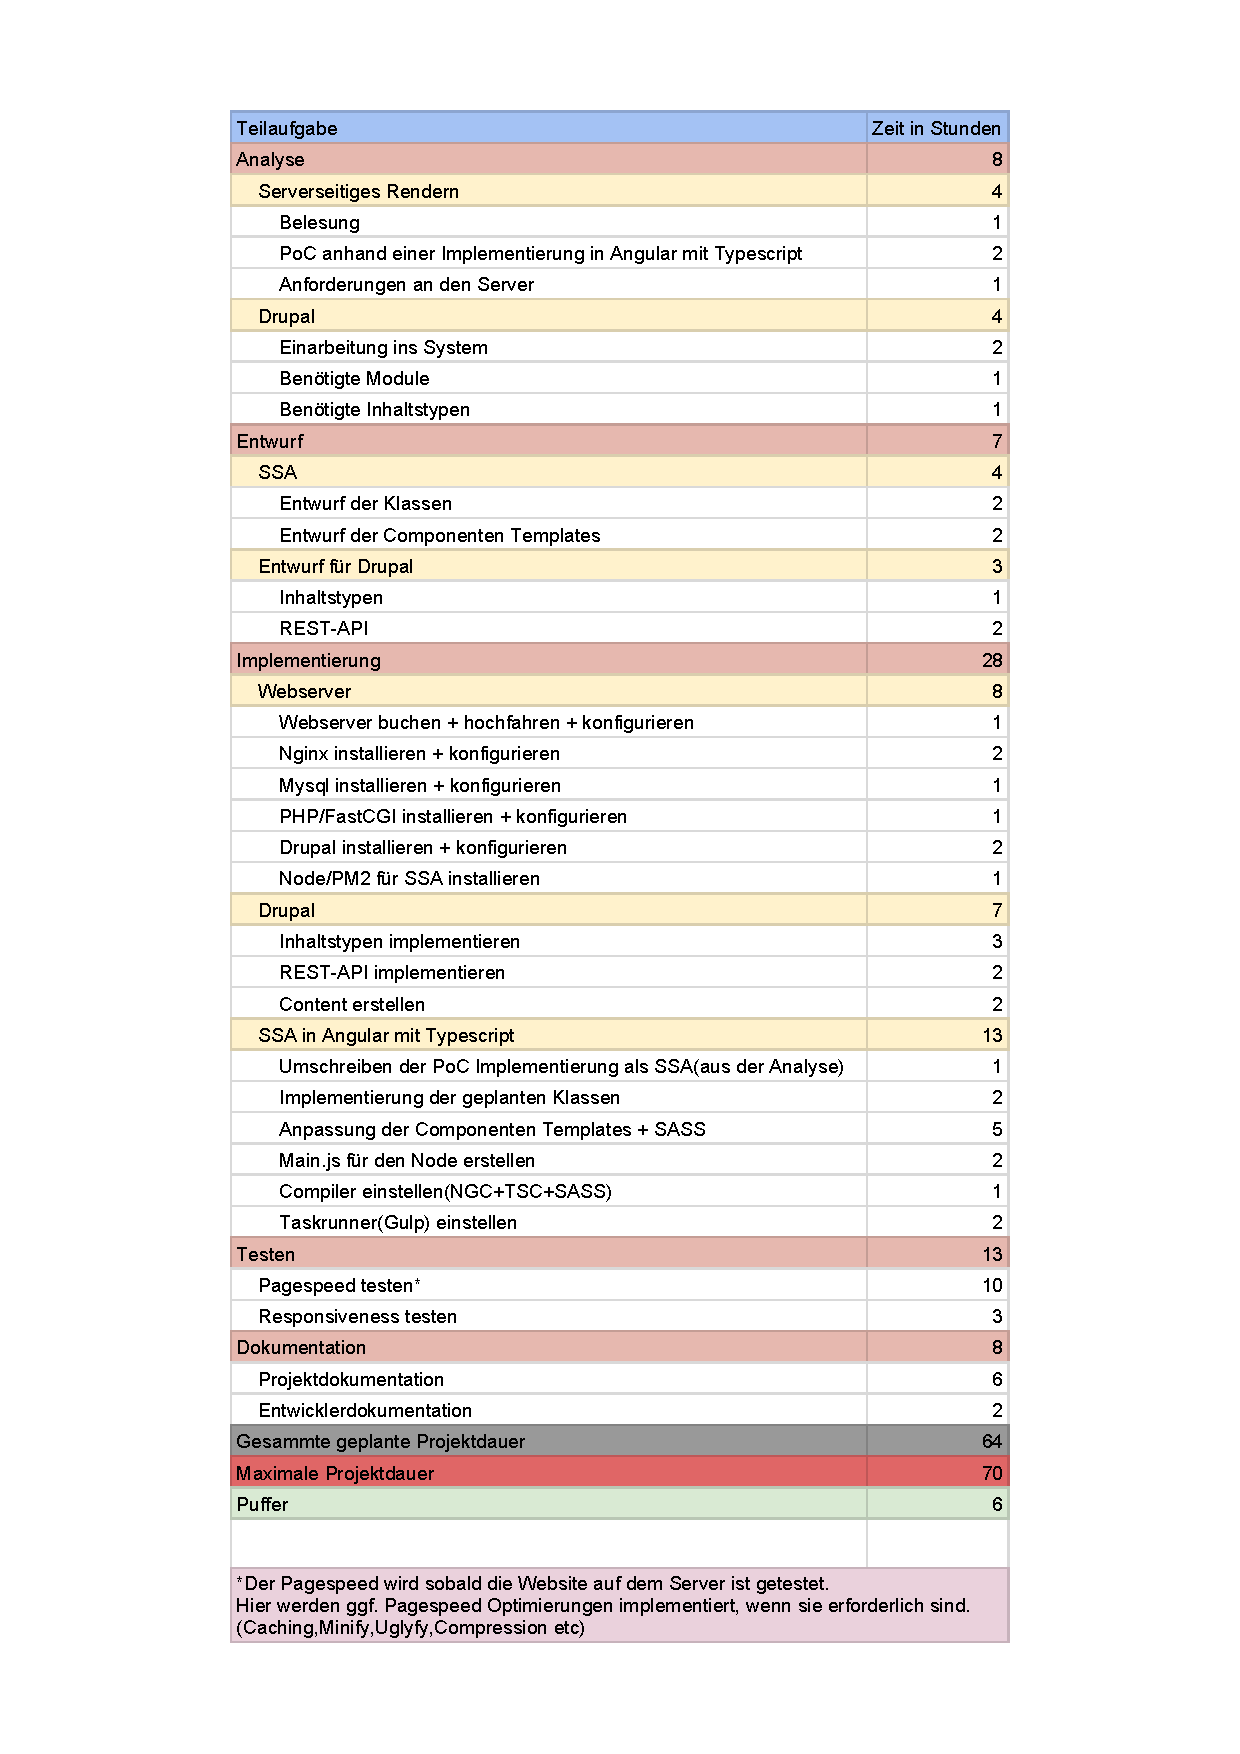
\includepdf[scale=0.7,pages=1,pagecommand=\section{Abbildungen}\subsection{Tabellen}\subsubsection{Detaillierte Übersicht der Aufgaben}\label{sec:teilaufg}]{Teilaufgaben}
\begin{landscape}
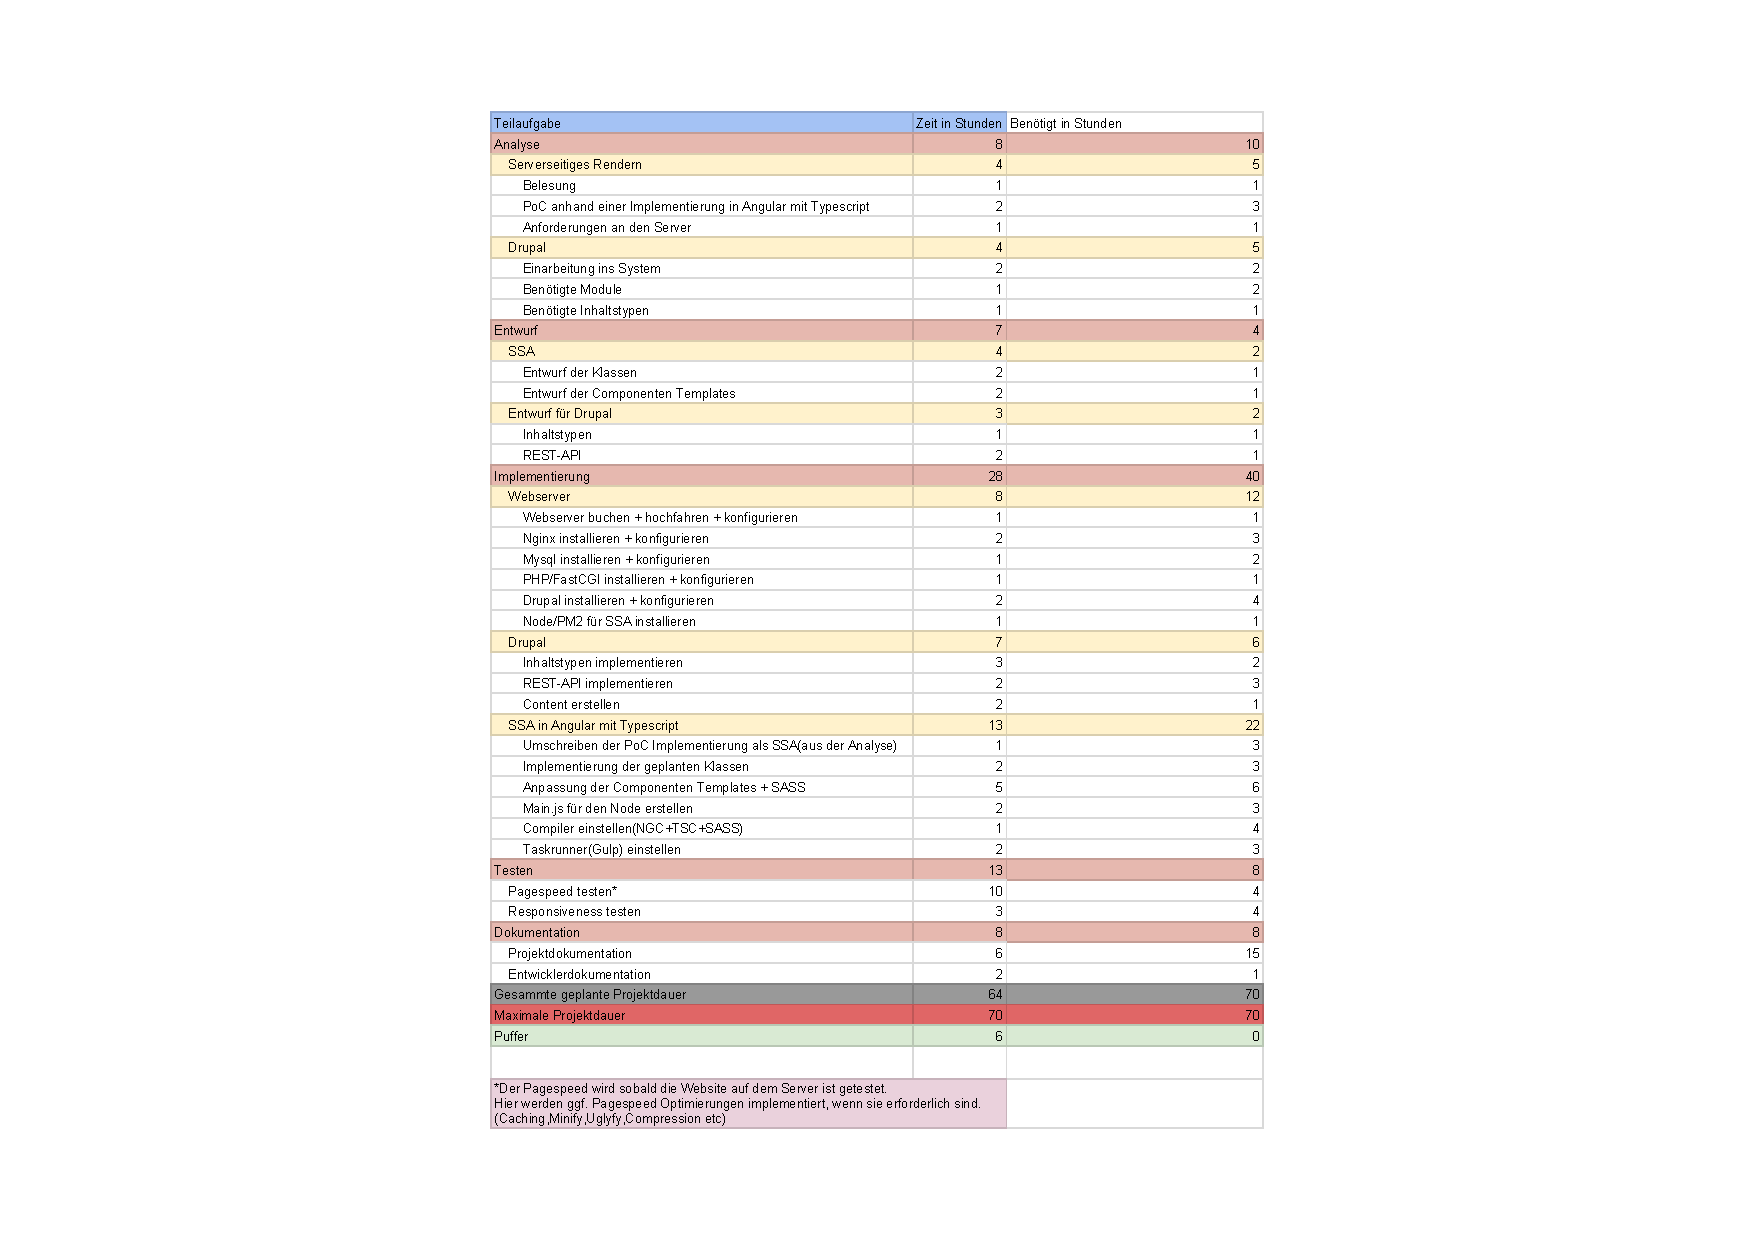
\includepdf[scale=1,pages=1,landscape=true,pagecommand=\subsubsection{Zeitplan}\label{sec:time}]{Zeitplan}
\end{landscape}
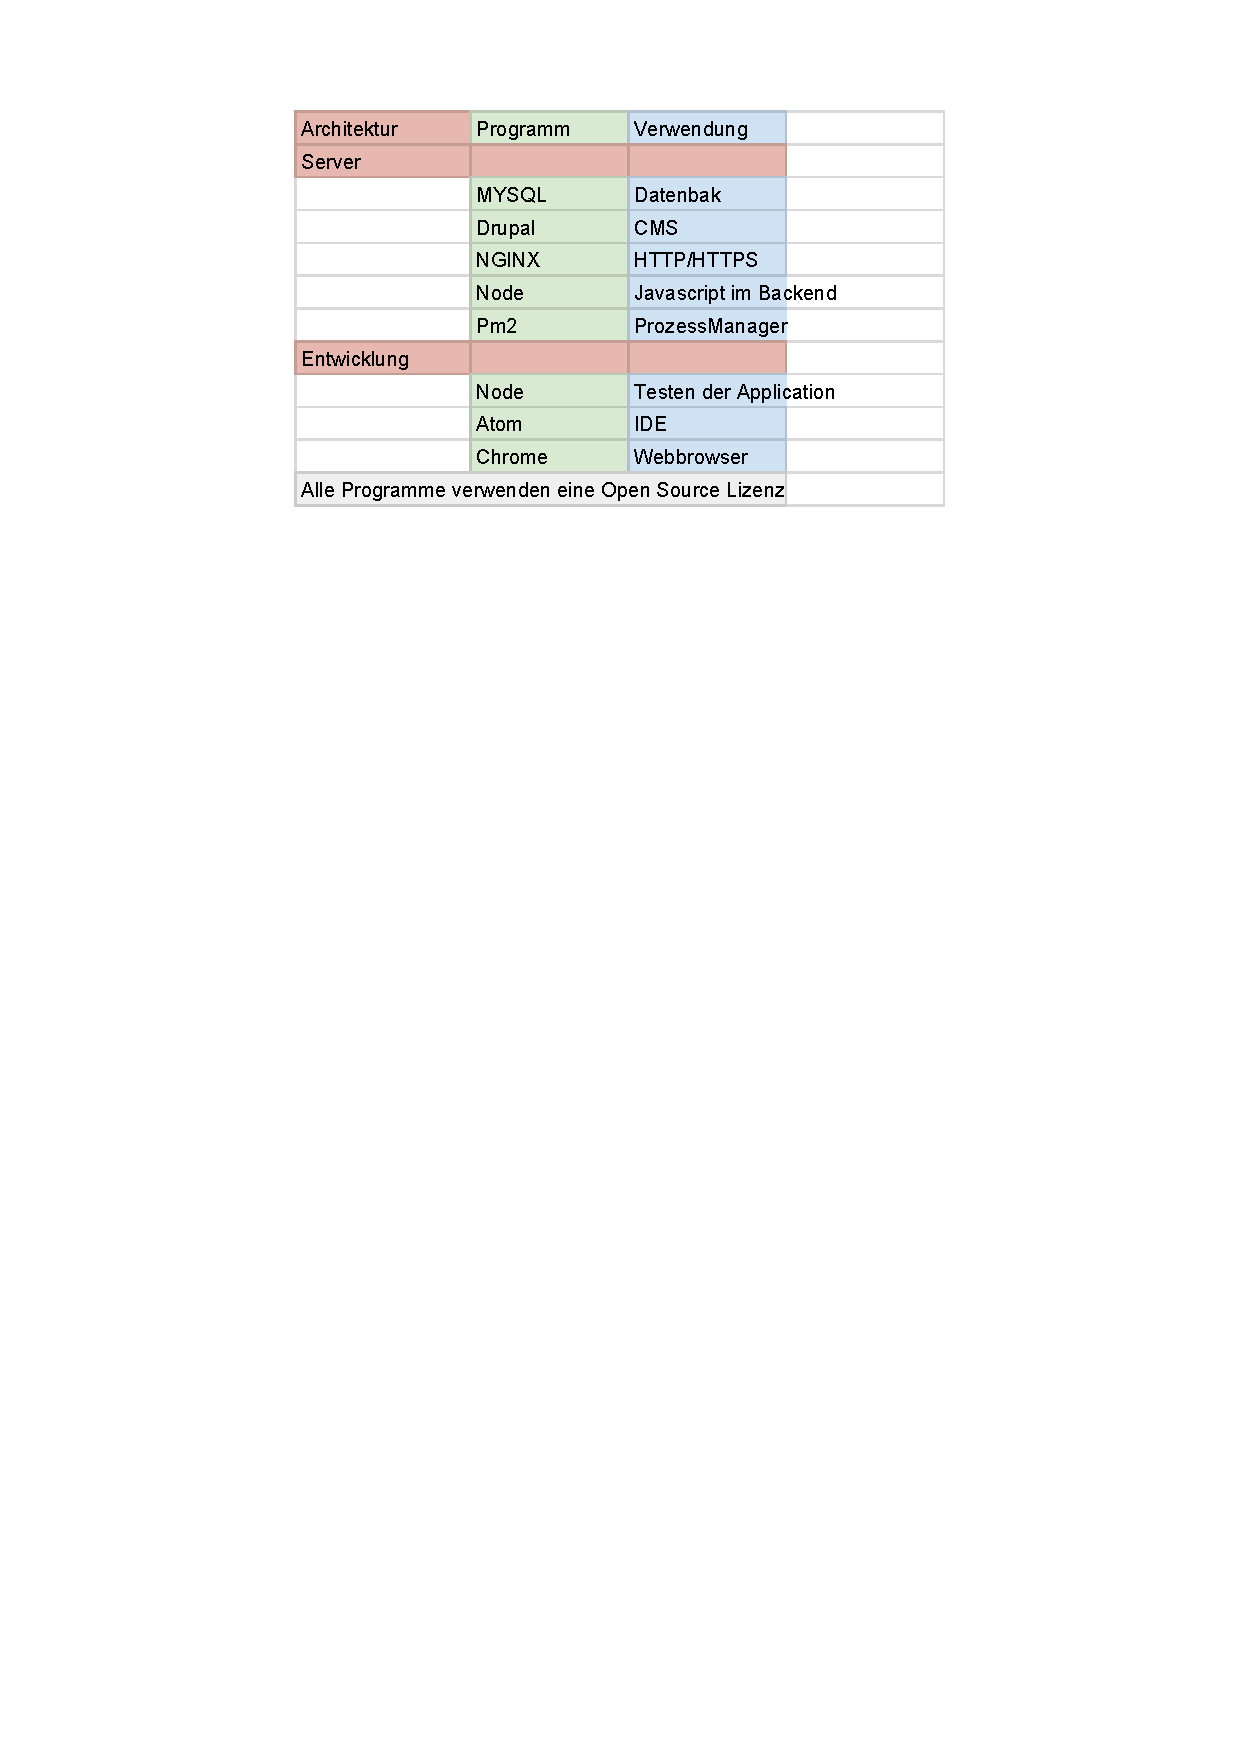
\includepdf[scale=0.8,pages=1,pagecommand=\subsubsection{Programme}\label{sec:progs}]{programme}
\subsection{Grafiken}
\subsubsection{Aufbau der Seite}
\label{sec:epage}
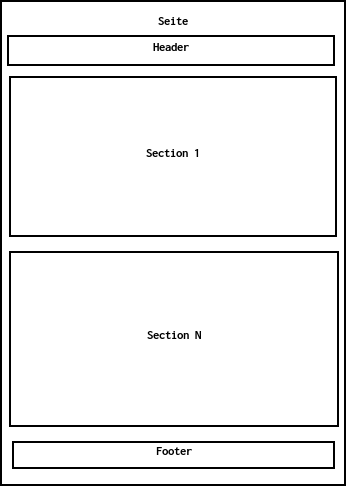
\includegraphics[scale=0.5,height=10cm]{Seite}
\subsubsection{Projekt Architektur}
\label{sec:eprojekt}
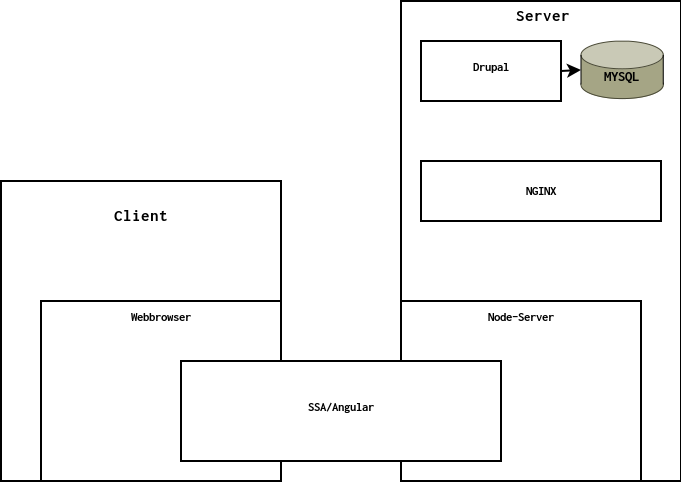
\includegraphics[scale=0.5,height=10cm]{Entwurf}
\subsubsection{SSR Node Entwurf}
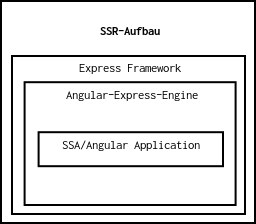
\includegraphics[scale=1]{SSR}
\label{sec:essr}
\subsubsection{SPA Entwurf}
\label{sec:espa}
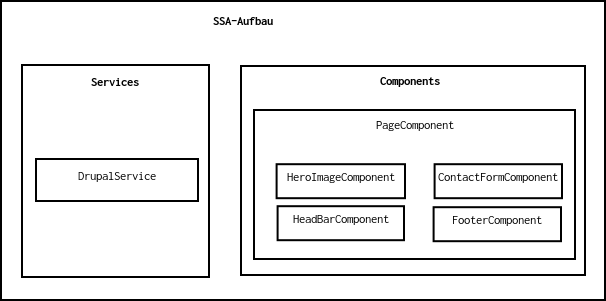
\includegraphics[scale=0.7]{SSA}
\subsubsection{Website Mockup}
\label{sec:mockup}
\centering
Aufgrund der Größenlimitierung der PDF muss das Bild im Webbrowser Aufgerufen werden.\\
https://goo.gl/qfjDmC
\flushleft
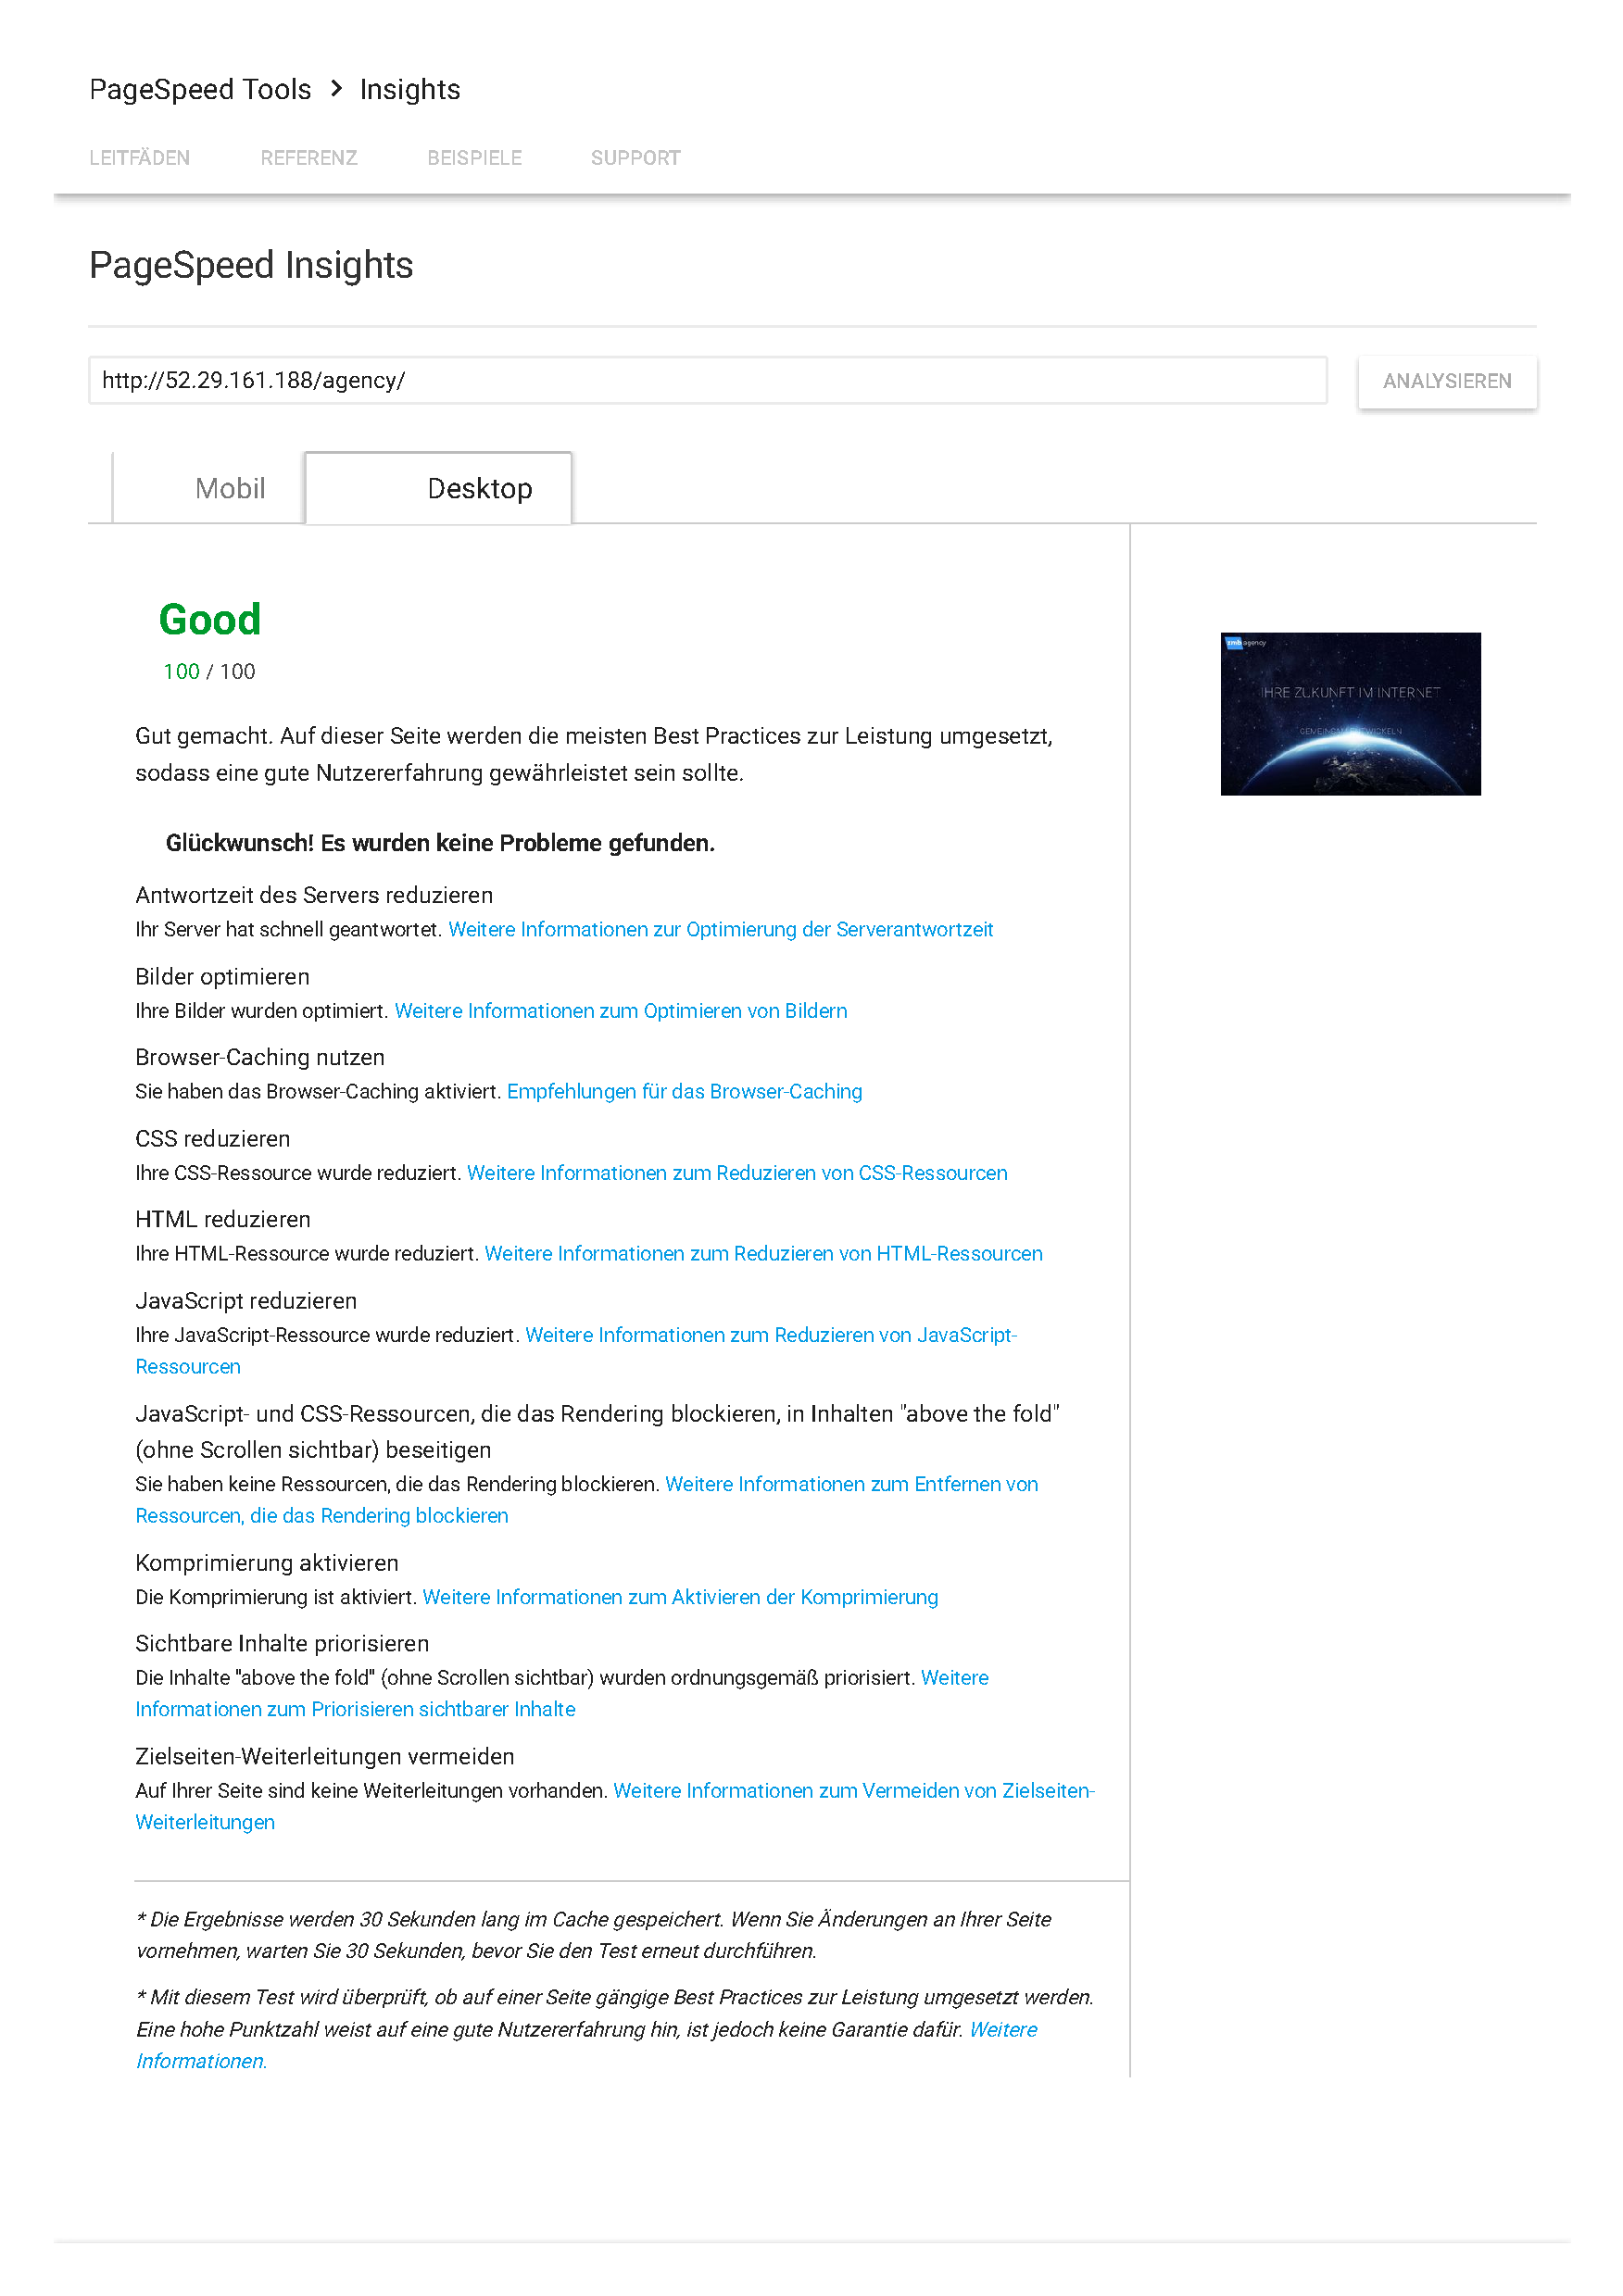
\includepdf[scale=0.8,pages=1,pagecommand=\subsubsection{PageSpeed Insights}\label{sec:google}]{pagespeed}
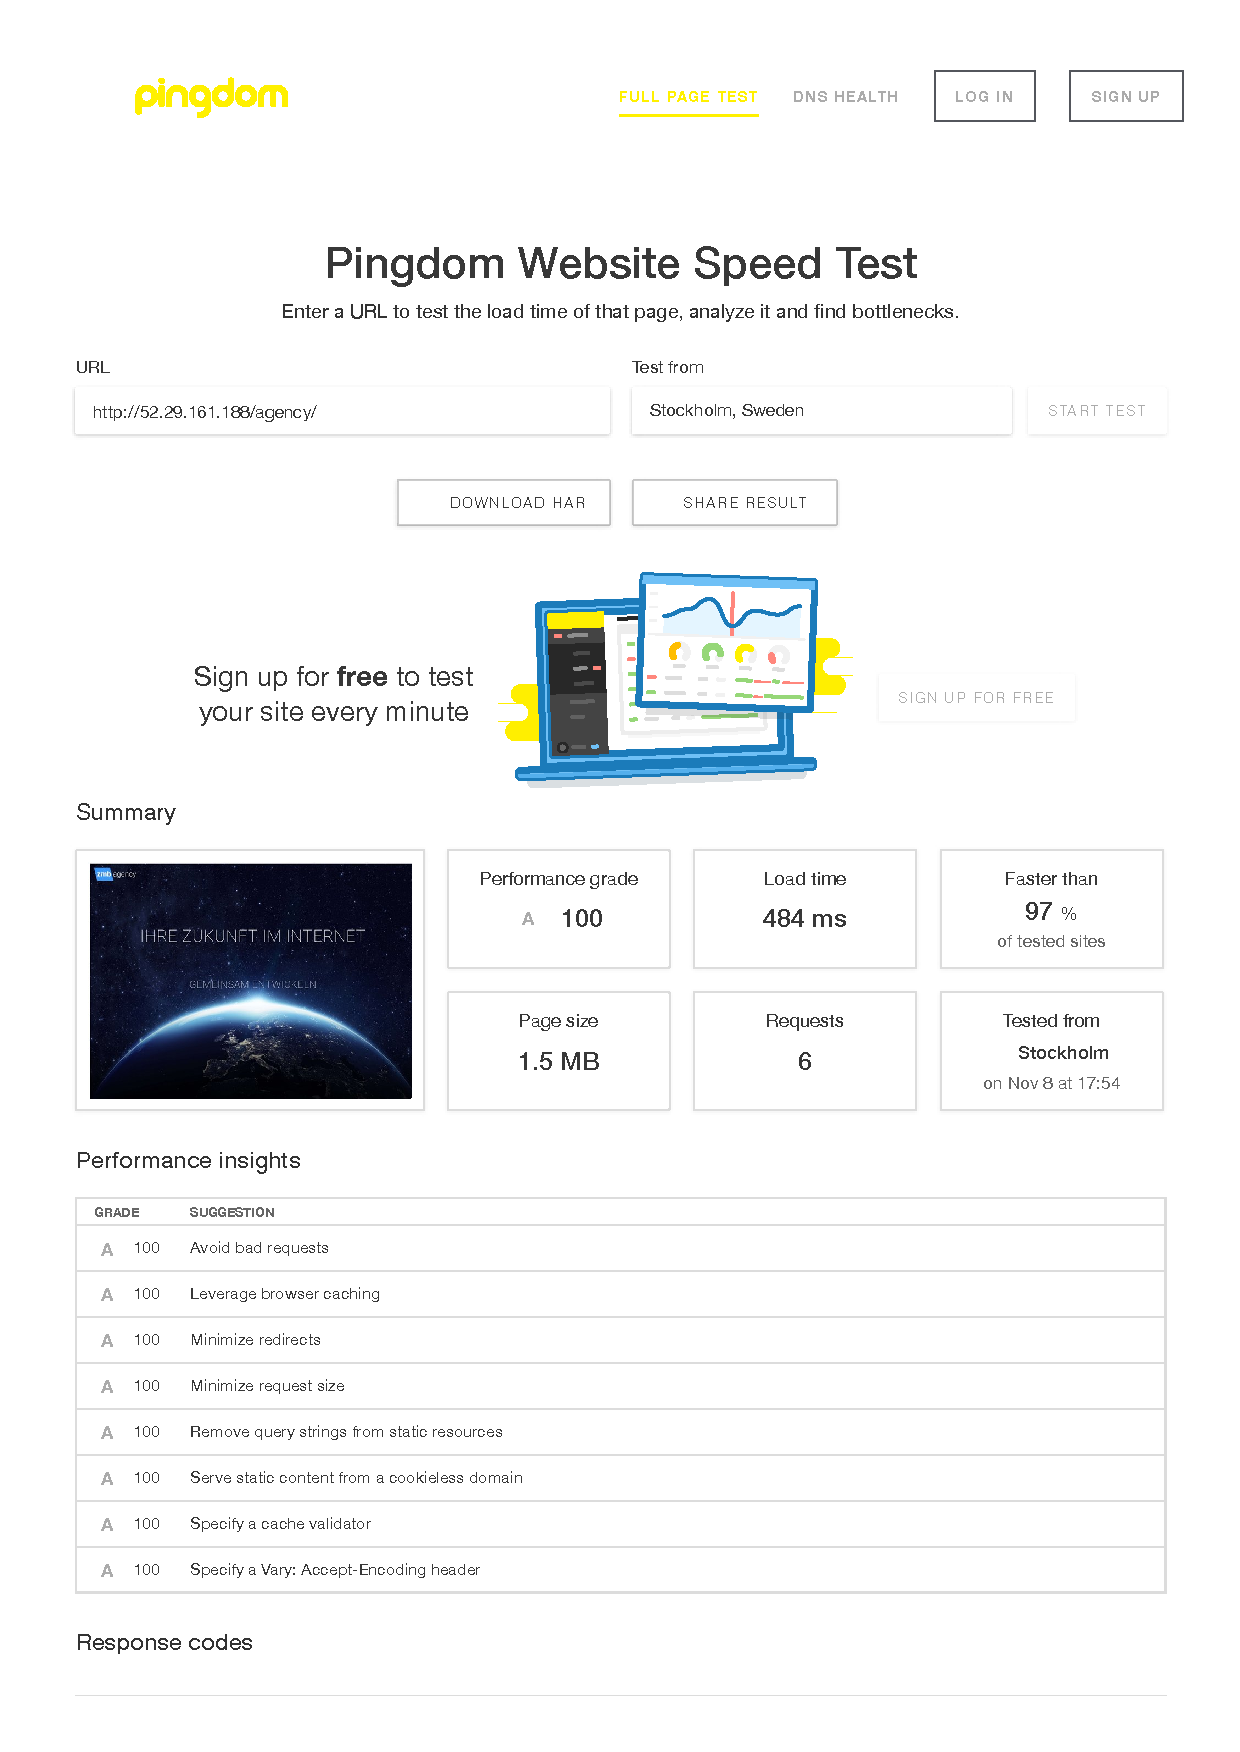
\includepdf[scale=0.8,pages=1,pagecommand=\subsubsection{Pingdom}\label{sec:pingdom}]{pingdom}
\subsection{Screenshots}
\subsubsection{Audit}
\label{sec:audit}
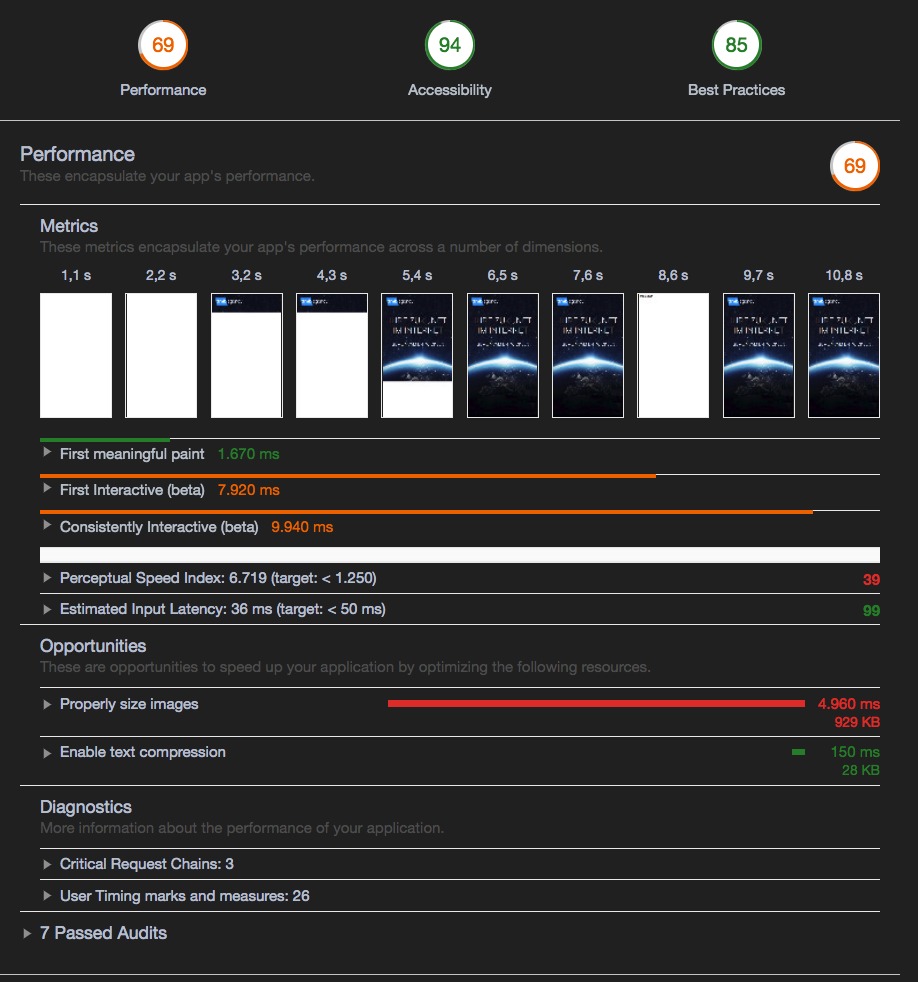
\includegraphics[scale=0.5]{audit}
\subsubsection{REST Schnittstellen Drupal}
\label{sec:rest}
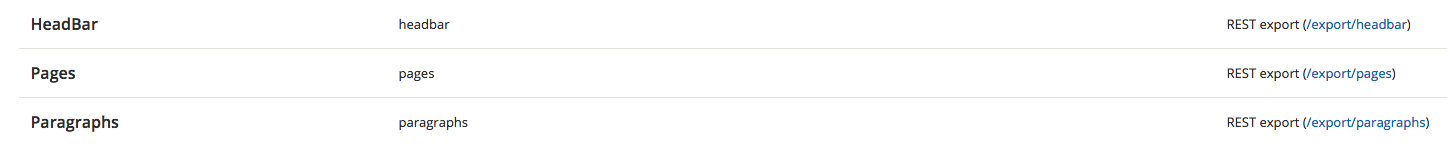
\includegraphics[width=16cm]{Rest}
\subsubsection{Drupal Inhalte}
\label{sec:content}
\subsubsection*{Seite als Inhaltstyp}
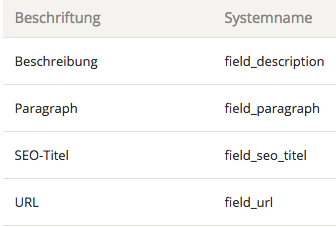
\includegraphics[scale=0.5]{Page}
\subsubsection*{Formular Sektion als Inhaltstyp}
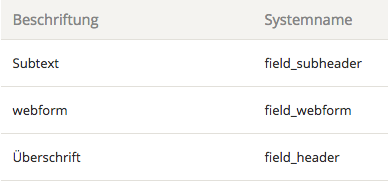
\includegraphics[scale=0.5]{Form}
\subsubsection*{Hero als Inhaltstyp}
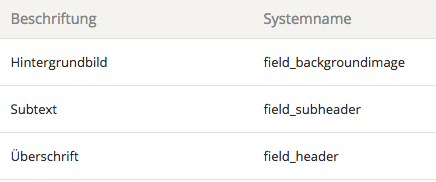
\includegraphics[scale=0.5]{Hero}
\subsubsection{Alte Website}
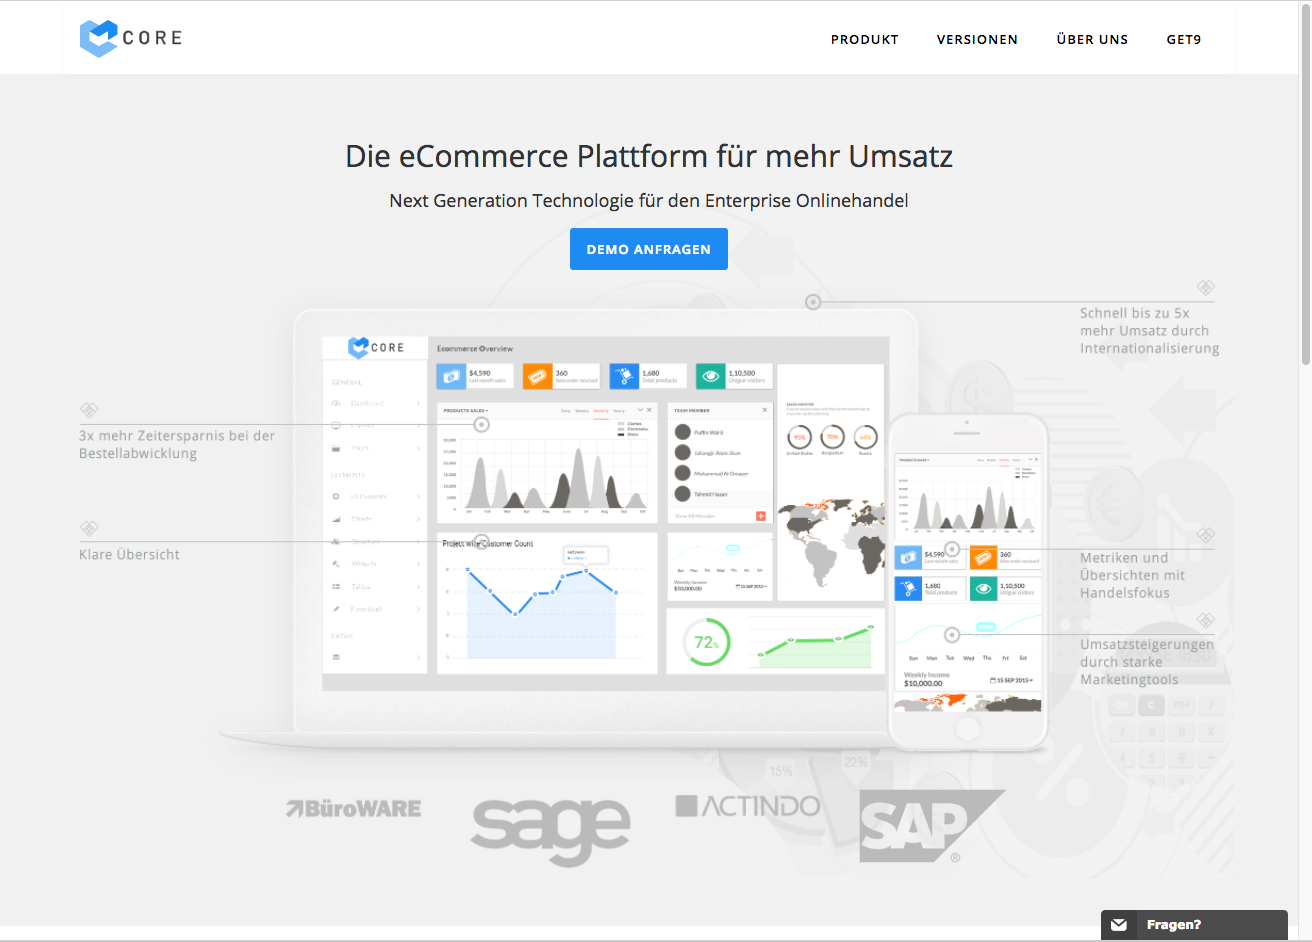
\includegraphics[scale=0.3]{getcore}
\subsubsection{Entwickler Dokumentation}
\label{sec:doku}
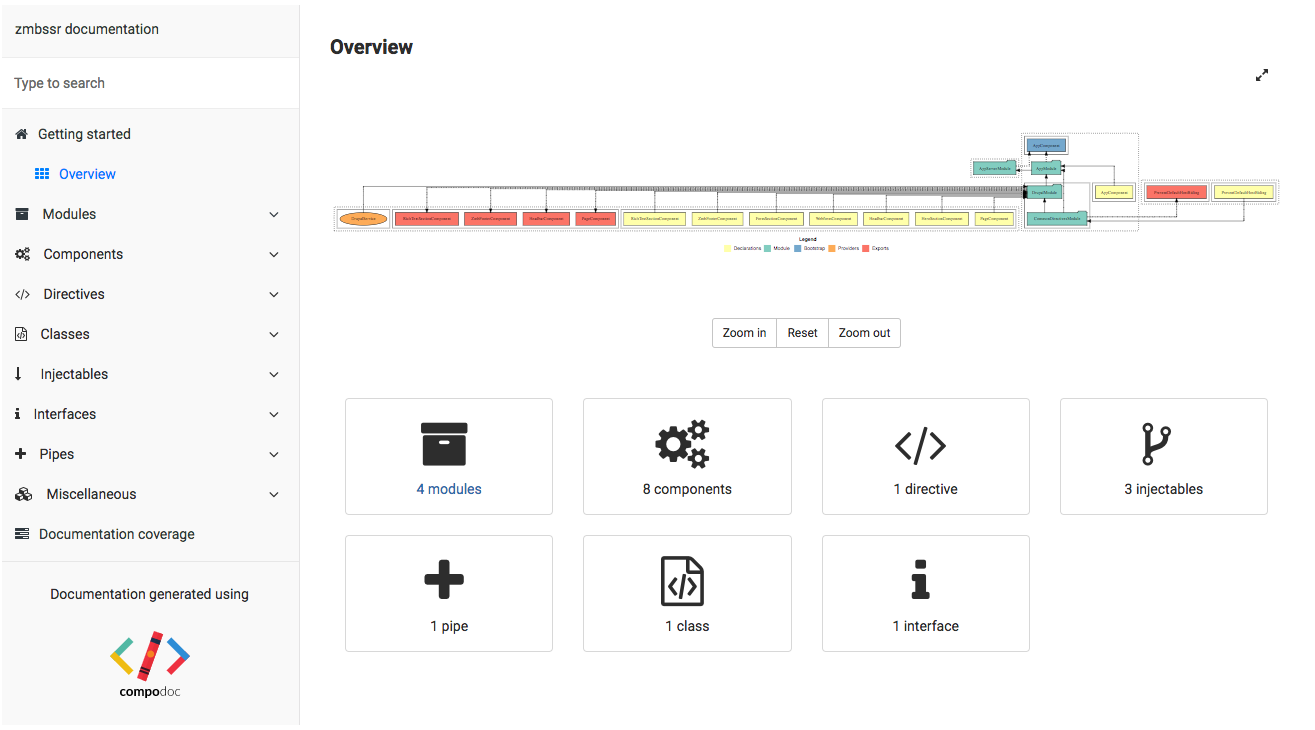
\includegraphics[scale=0.3]{compodoc}
\subsubsection{Ordner Struktur}
\label{sec:ordner}
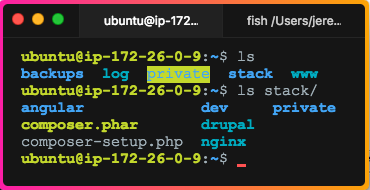
\includegraphics[scale=0.8]{terminal}
\subsubsection{Responsive Design}
\label{sec:responsive}
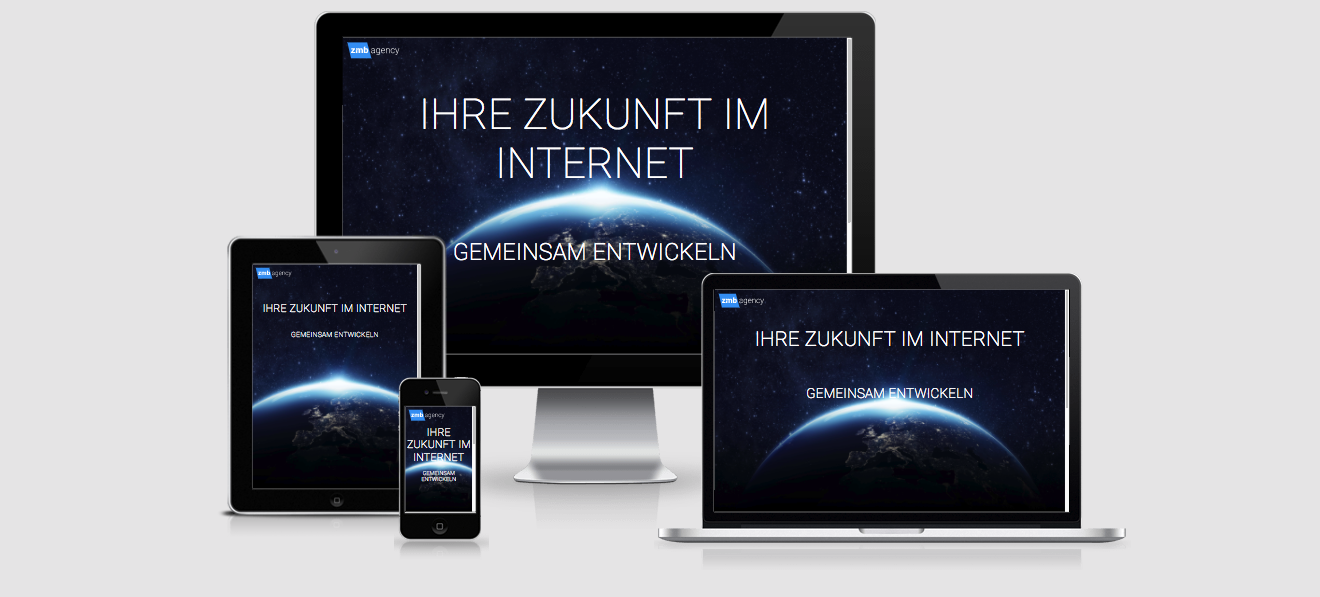
\includegraphics[scale=0.3]{responsive}
\section{Code Beispiele}
\subsection{NGINX Konfiguration Auszug}
\label{sec:nginx}
\begin{lstlisting}[frame=single,   basicstyle=\footnotesize]
location  / {
        proxy_pass http://localhost:1337/;
        proxy_http_version 1.1;
        proxy_set_header Upgrade $http_upgrade;
        proxy_set_header Connection 'upgrade';
        proxy_set_header Host $host;
        proxy_cache_bypass $http_upgrade;
    }

location /drupal/ {
        index index.php;
        root /data/www/drupal;
    }
\end{lstlisting}
\end{appendices}
\end{document}
